\subsection{Contexto Económico}\subsubsection{Producto Interno Bruto}

El PIB
\footnote{Producto Interno Bruto a precios de comprador, en millones de guaraníes constantes de 2014.}
del Paraguay ha crecido en promedio a un ritmo del 3,5\% anual entre los
años 2009 y 2020, donde se destacan dos picos de crecimiento en los a
ños 2010 y 2013 y dos de contracción de la economía en los años 2009 y
2012. Considerando los últimos 5 años el crecimiento ha sido sostenido y
en torno al 2,3\%.

El PIB del año 2020 da cuenta de un decrecimiento económico del orden
del 0,6\%
\footnote{Anexo Estadístico del Informe Económico del BCP. Departamento de Estadísticas del Sector Real.},
esto concuerda con la declaración de estado de emergencia en todo el
territorio nacional ante la pandemia declarada por la Organización
Mundial de la Salud a causa del COVID-19 o CORONAVIRUS, la cual ha
traído consigo innumerables crisis asociadas, tanto en el ámbito
sanitario como en el económico y social.

\begin{figure}[H]
\begin{center}
                    \caption{PIB a precios corrientes y constantes}
                    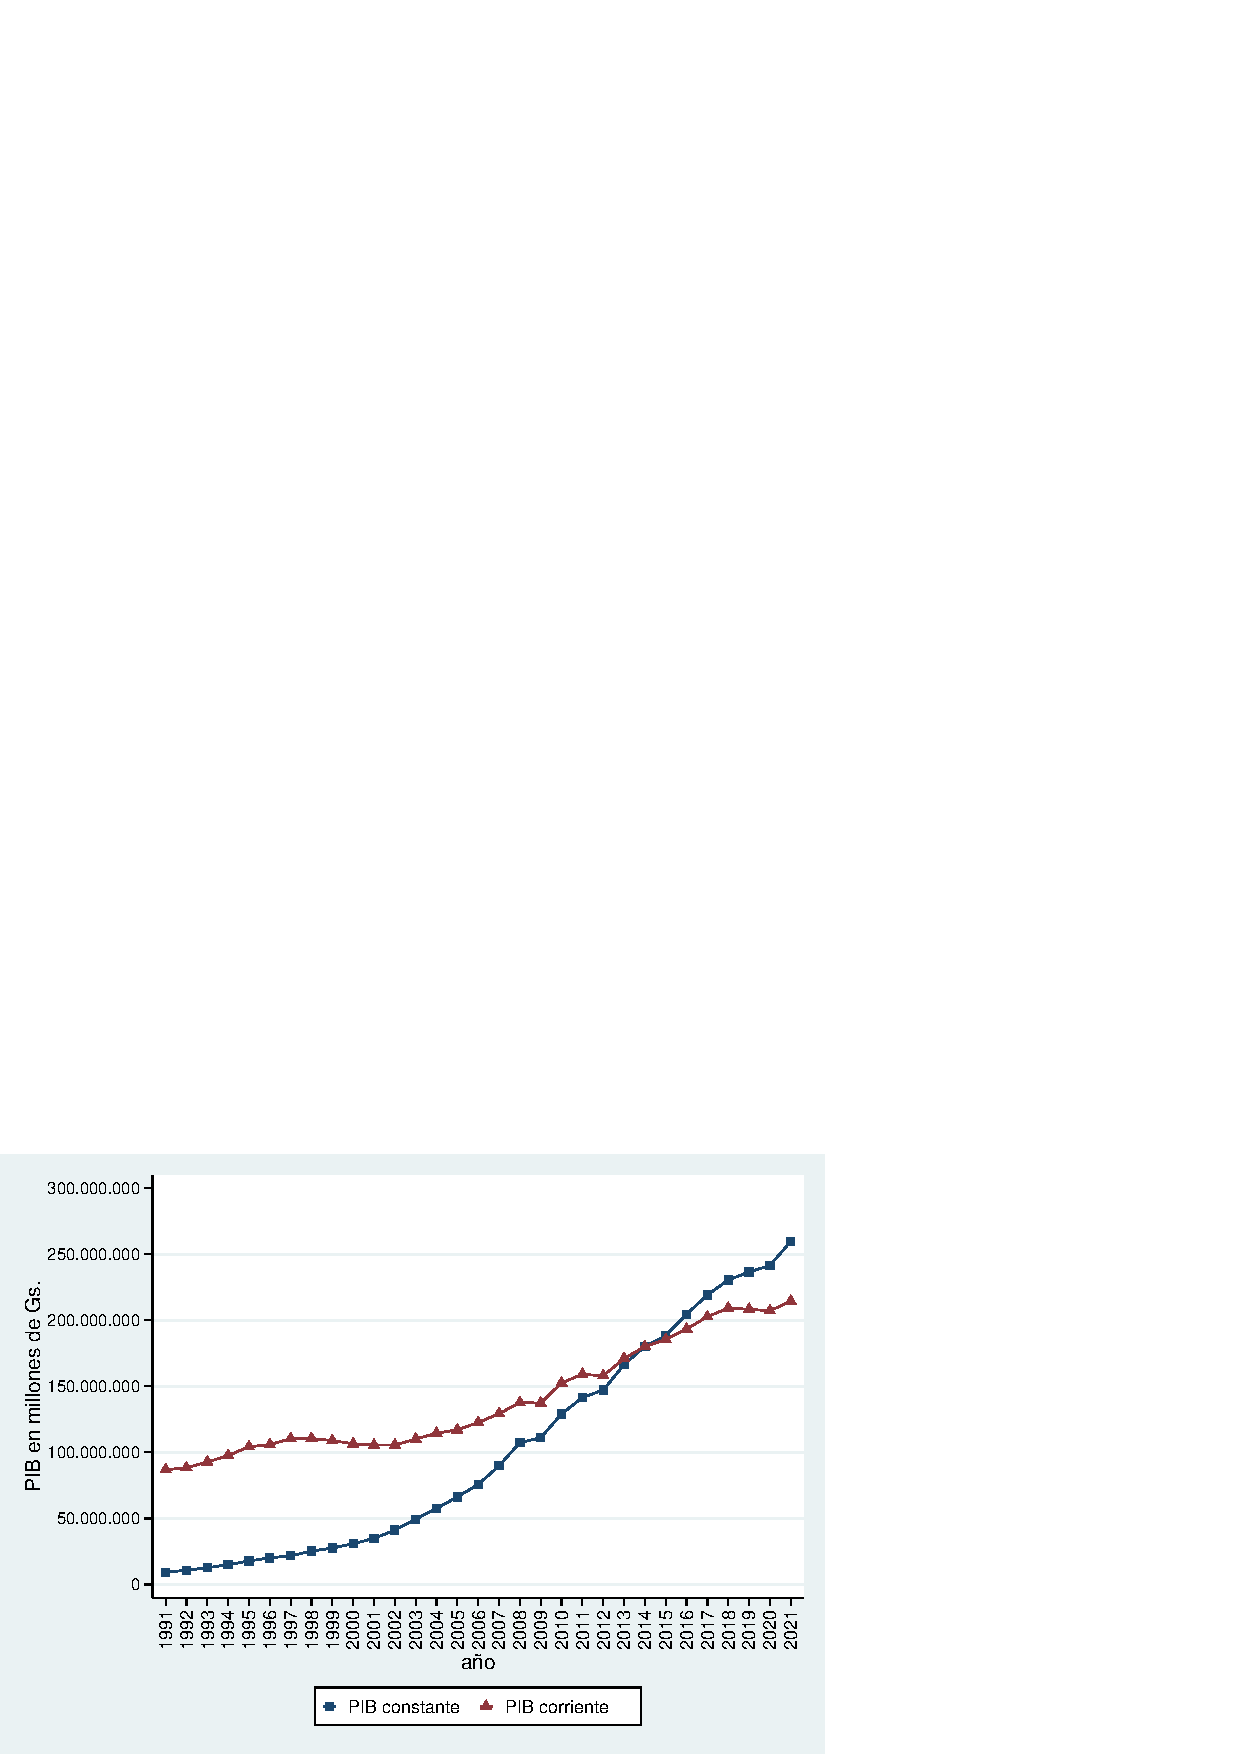
\includegraphics[scale=0.55]{BCP_pib_corr_cte.png}
                                    \item \footnotesize Fuente : Banco Central del Paraguay. 
                                    \item \footnotesize Nota : 
                    \end{center}
\end{figure}

\begin{figure}[H]
\begin{center}
                    \caption{Variación interanual del PIB a precios constantes. Periodo 1991-2021}
                    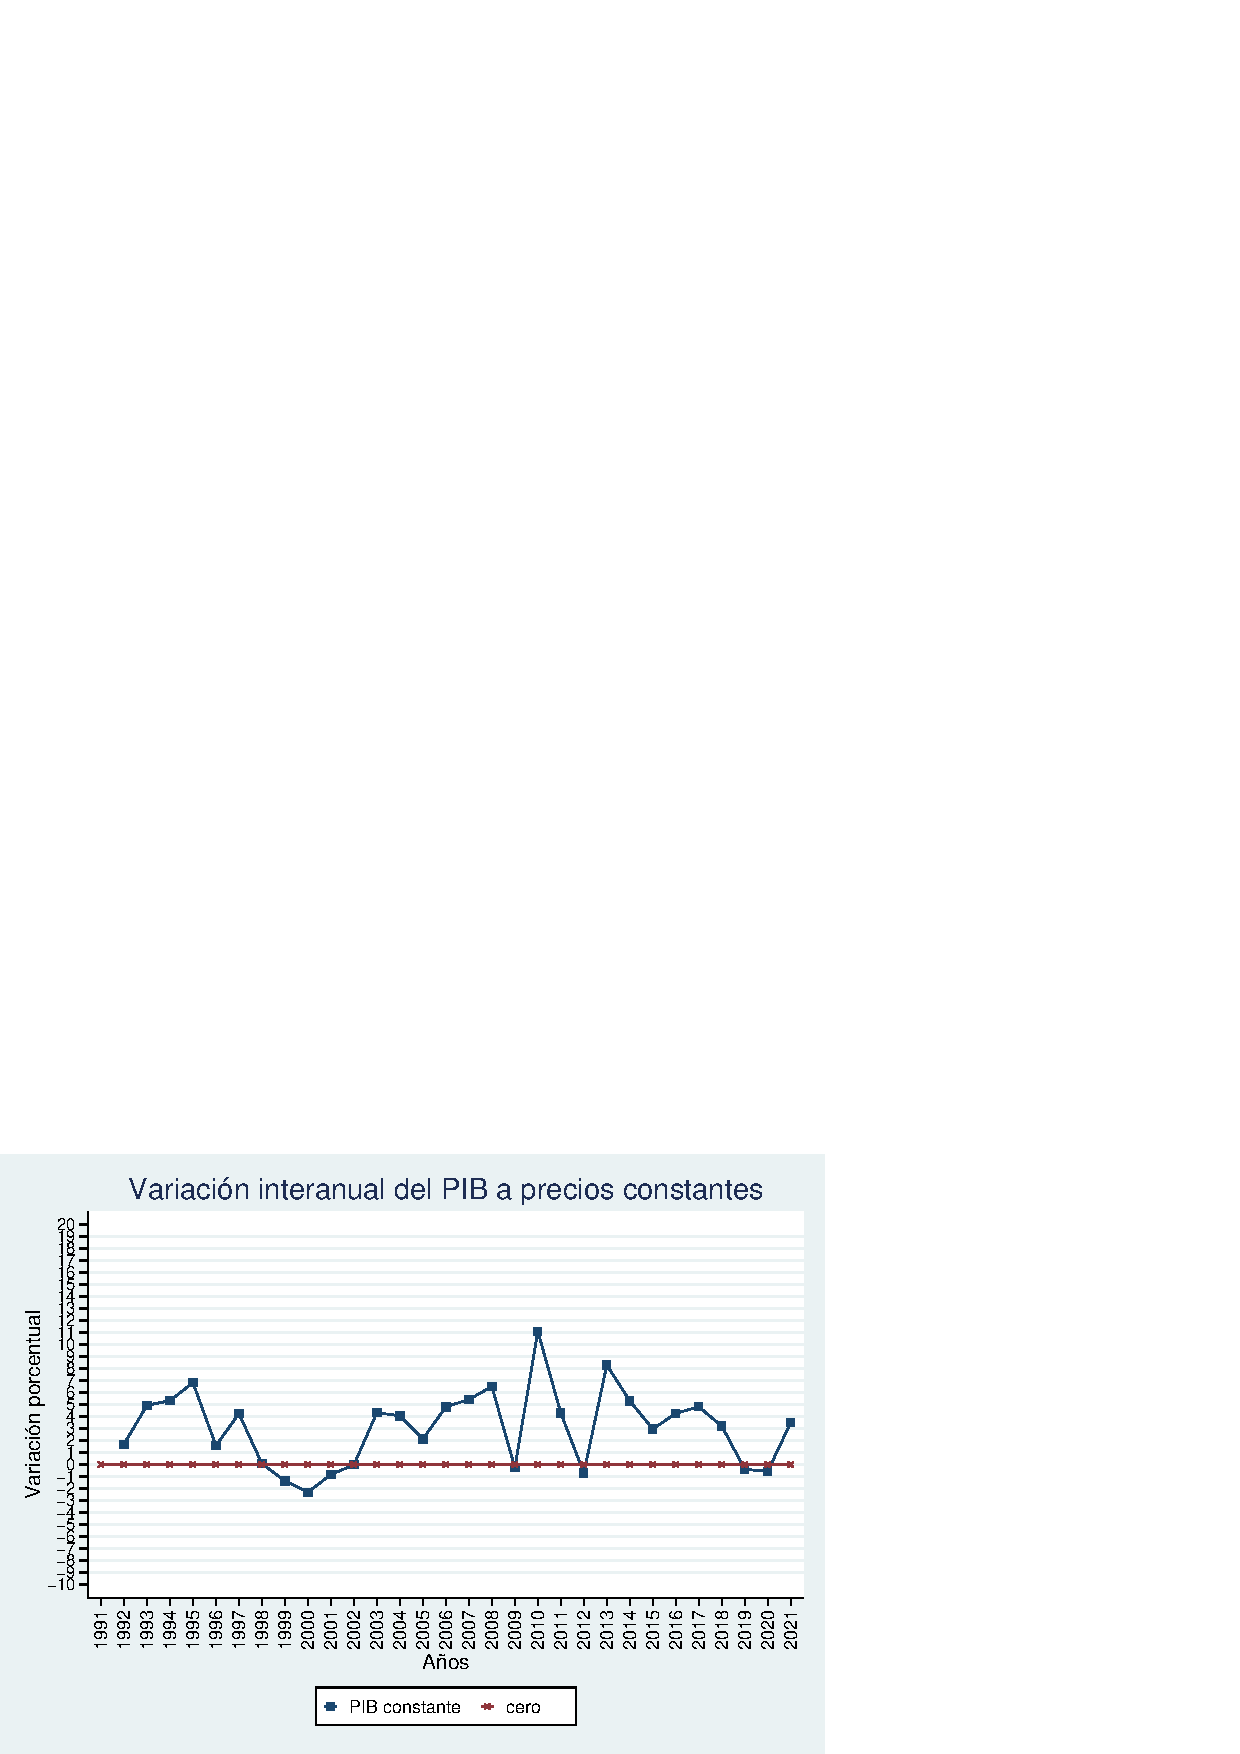
\includegraphics[scale=0.55]{BCP_var_pibcte.png}
                                    \item \footnotesize Fuente : Banco Central del Paraguay. 
                                    %\item \footnotesize Nota : 
                    \end{center}
\end{figure}

\begin{table}[H]
\begin{center}
\scriptsize
\caption{\bf{PIB a precios corrientes y constantes. Periodo 1991-2021}}
\begin{tabular}{l|rrrrrr}
\begin{tabular}{llll}
\cline{1-4}
\multicolumn{1}{c}{} &
  \multicolumn{1}{|r}{PIB\_constantes} &
  \multicolumn{1}{r}{PIB\_corrientes} &
  \multicolumn{1}{r}{Variación del PIB\_contante} \\
\cline{1-4}
\multicolumn{1}{l}{Año} &
  \multicolumn{1}{|r}{} &
  \multicolumn{1}{r}{} &
  \multicolumn{1}{r}{} \\
\multicolumn{1}{l}{\hspace{1em}1991} &
  \multicolumn{1}{|r}{86.864.501,40} &
  \multicolumn{1}{r}{9.255.684,16} &
  \multicolumn{1}{r}{0,00} \\
\multicolumn{1}{l}{\hspace{1em}1992} &
  \multicolumn{1}{|r}{88.338.095,13} &
  \multicolumn{1}{r}{10.738.283,27} &
  \multicolumn{1}{r}{1,70} \\
\multicolumn{1}{l}{\hspace{1em}1993} &
  \multicolumn{1}{|r}{92.698.781,01} &
  \multicolumn{1}{r}{12.645.361,49} &
  \multicolumn{1}{r}{4,94} \\
\multicolumn{1}{l}{\hspace{1em}1994} &
  \multicolumn{1}{|r}{97.628.425,86} &
  \multicolumn{1}{r}{14.992.331,68} &
  \multicolumn{1}{r}{5,32} \\
\multicolumn{1}{l}{\hspace{1em}1995} &
  \multicolumn{1}{|r}{104.289.428,16} &
  \multicolumn{1}{r}{17.789.145,33} &
  \multicolumn{1}{r}{6,82} \\
\multicolumn{1}{l}{\hspace{1em}1996} &
  \multicolumn{1}{|r}{105.930.719,67} &
  \multicolumn{1}{r}{20.132.862,10} &
  \multicolumn{1}{r}{1,57} \\
\multicolumn{1}{l}{\hspace{1em}1997} &
  \multicolumn{1}{|r}{110.424.847,51} &
  \multicolumn{1}{r}{21.702.866,40} &
  \multicolumn{1}{r}{4,24} \\
\multicolumn{1}{l}{\hspace{1em}1998} &
  \multicolumn{1}{|r}{110.499.978,10} &
  \multicolumn{1}{r}{25.248.610,40} &
  \multicolumn{1}{r}{0,07} \\
\multicolumn{1}{l}{\hspace{1em}1999} &
  \multicolumn{1}{|r}{108.990.460,31} &
  \multicolumn{1}{r}{27.563.440,66} &
  \multicolumn{1}{r}{-1,37} \\
\multicolumn{1}{l}{\hspace{1em}2000} &
  \multicolumn{1}{|r}{106.468.267,86} &
  \multicolumn{1}{r}{30.874.087,61} &
  \multicolumn{1}{r}{-2,31} \\
\multicolumn{1}{l}{\hspace{1em}2001} &
  \multicolumn{1}{|r}{105.580.264,25} &
  \multicolumn{1}{r}{34.883.186,50} &
  \multicolumn{1}{r}{-0,83} \\
\multicolumn{1}{l}{\hspace{1em}2002} &
  \multicolumn{1}{|r}{105.557.665,43} &
  \multicolumn{1}{r}{41.135.696,94} &
  \multicolumn{1}{r}{-0,02} \\
\multicolumn{1}{l}{\hspace{1em}2003} &
  \multicolumn{1}{|r}{110.118.543,49} &
  \multicolumn{1}{r}{49.411.959,70} &
  \multicolumn{1}{r}{4,32} \\
\multicolumn{1}{l}{\hspace{1em}2004} &
  \multicolumn{1}{|r}{114.586.513,50} &
  \multicolumn{1}{r}{57.501.991,73} &
  \multicolumn{1}{r}{4,06} \\
\multicolumn{1}{l}{\hspace{1em}2005} &
  \multicolumn{1}{|r}{117.031.206,07} &
  \multicolumn{1}{r}{66.335.828,41} &
  \multicolumn{1}{r}{2,13} \\
\multicolumn{1}{l}{\hspace{1em}2006} &
  \multicolumn{1}{|r}{122.657.033,30} &
  \multicolumn{1}{r}{75.681.657,80} &
  \multicolumn{1}{r}{4,81} \\
\multicolumn{1}{l}{\hspace{1em}2007} &
  \multicolumn{1}{|r}{129.307.035,07} &
  \multicolumn{1}{r}{89.866.048,80} &
  \multicolumn{1}{r}{5,42} \\
\multicolumn{1}{l}{\hspace{1em}2008} &
  \multicolumn{1}{|r}{137.707.197,80} &
  \multicolumn{1}{r}{107.403.590,63} &
  \multicolumn{1}{r}{6,50} \\
\multicolumn{1}{l}{\hspace{1em}2009} &
  \multicolumn{1}{|r}{137.347.592,90} &
  \multicolumn{1}{r}{111.030.933,59} &
  \multicolumn{1}{r}{-0,26} \\
\multicolumn{1}{l}{\hspace{1em}2010} &
  \multicolumn{1}{|r}{152.586.625,97} &
  \multicolumn{1}{r}{129.092.883,48} &
  \multicolumn{1}{r}{11,10} \\
\multicolumn{1}{l}{\hspace{1em}2011} &
  \multicolumn{1}{|r}{159.127.055,18} &
  \multicolumn{1}{r}{141.486.449,39} &
  \multicolumn{1}{r}{4,29} \\
\multicolumn{1}{l}{\hspace{1em}2012} &
  \multicolumn{1}{|r}{158.000.367,02} &
  \multicolumn{1}{r}{147.225.506,09} &
  \multicolumn{1}{r}{-0,71} \\
\multicolumn{1}{l}{\hspace{1em}2013} &
  \multicolumn{1}{|r}{171.103.458,31} &
  \multicolumn{1}{r}{166.350.805,11} &
  \multicolumn{1}{r}{8,29} \\
\multicolumn{1}{l}{\hspace{1em}2014} &
  \multicolumn{1}{|r}{180.174.060,88} &
  \multicolumn{1}{r}{180.174.060,97} &
  \multicolumn{1}{r}{5,30} \\
\multicolumn{1}{l}{\hspace{1em}2015} &
  \multicolumn{1}{|r}{185.502.081,24} &
  \multicolumn{1}{r}{188.477.326,98} &
  \multicolumn{1}{r}{2,96} \\
\multicolumn{1}{l}{\hspace{1em}2016} &
  \multicolumn{1}{|r}{193.419.357,99} &
  \multicolumn{1}{r}{204.647.273,08} &
  \multicolumn{1}{r}{4,27} \\
\multicolumn{1}{l}{\hspace{1em}2017} &
  \multicolumn{1}{|r}{202.722.981,63} &
  \multicolumn{1}{r}{219.122.277,20} &
  \multicolumn{1}{r}{4,81} \\
\multicolumn{1}{l}{\hspace{1em}2018} &
  \multicolumn{1}{|r}{209.218.733,46} &
  \multicolumn{1}{r}{230.576.477,47} &
  \multicolumn{1}{r}{3,20} \\
\multicolumn{1}{l}{\hspace{1em}2019} &
  \multicolumn{1}{|r}{208.377.977,31} &
  \multicolumn{1}{r}{236.566.703,63} &
  \multicolumn{1}{r}{-0,40} \\
\multicolumn{1}{l}{\hspace{1em}2020} &
  \multicolumn{1}{|r}{207.199.192,58} &
  \multicolumn{1}{r}{241.527.085,72} &
  \multicolumn{1}{r}{-0,57} \\
\multicolumn{1}{l}{\hspace{1em}2021} &
  \multicolumn{1}{|r}{214.451.164,32} &
  \multicolumn{1}{r}{259.745.767,58} &
  \multicolumn{1}{r}{3,50} \\
\cline{1-4}
\end{tabular}

\end{tabular}
                    \item \footnotesize Fuente : Banco Central del Paraguay. 
                    %\item \footnotesize Nota : 
\end{center}
\end{table}

\subsubsection{Inflación}

La
inflación\footnote{Índice de Precios al Consumidor. Base diciembre de 2017=100.}
, en economía, es el aumento generalizado y sostenido de los precios de
los bienes y servicios existentes en el mercado durante un período de
tiempo, y uno de los mecani smos para medir la variación de precios en
el Paraguay es a través del Índice de Precios al Consumidor (IPC) del
Área Metropolitana de Asunción elaborado por el BCP, el cual mide la
evolución de los precios (en promedio) de un conjunto de bienes y servi
cios representativos del gasto de consumo de los hogares (una canasta).

La inflación del año 2020 ha ascendido a 2,2\% por debajo del 2,8\%
registrado en al año 2019. En tanto que la inflación interanual a julio
de 2021 ascendió a 5,2\%, superior a la tasa del 4,5\% registrada en
junio del corriente año \footnote{Informe de
 Inflación (IPC)-Julio 2021.}. Pese a esto, la variación aún se sitúa
dentro del rango objetivo a largo plazo establecido por el BCP de 4\% ±
2\% \footnote{Informe de Política Monetaria (Diciembre/2020)-BCP.}.

\begin{table}[H]
\begin{center}
\scriptsize
\caption{\bf{Evolución del Índice de Precios al Consumidor.}}
\begin{tabular}{l|rrrrrrrrrrrrrrr}
\begin{tabular}{lllllllllllll}
\cline{1-13}
\multicolumn{1}{c}{} &
  \multicolumn{12}{|c}{Mes} \\
\multicolumn{1}{c}{} &
  \multicolumn{1}{|r}{Ene} &
  \multicolumn{1}{r}{Feb} &
  \multicolumn{1}{r}{Mar} &
  \multicolumn{1}{r}{Abr} &
  \multicolumn{1}{r}{May} &
  \multicolumn{1}{r}{Jun} &
  \multicolumn{1}{r}{Jul} &
  \multicolumn{1}{r}{Ago} &
  \multicolumn{1}{r}{Sep} &
  \multicolumn{1}{r}{Oct} &
  \multicolumn{1}{r}{Nov} &
  \multicolumn{1}{r}{Dic} \\
\cline{1-13}
\multicolumn{1}{l}{Año} &
  \multicolumn{1}{|r}{} &
  \multicolumn{1}{r}{} &
  \multicolumn{1}{r}{} &
  \multicolumn{1}{r}{} &
  \multicolumn{1}{r}{} &
  \multicolumn{1}{r}{} &
  \multicolumn{1}{r}{} &
  \multicolumn{1}{r}{} &
  \multicolumn{1}{r}{} &
  \multicolumn{1}{r}{} &
  \multicolumn{1}{r}{} &
  \multicolumn{1}{r}{} \\
\multicolumn{1}{l}{\hspace{1em}2000} &
  \multicolumn{1}{|r}{32,86} &
  \multicolumn{1}{r}{33,33} &
  \multicolumn{1}{r}{34,02} &
  \multicolumn{1}{r}{34,31} &
  \multicolumn{1}{r}{34,44} &
  \multicolumn{1}{r}{34,24} &
  \multicolumn{1}{r}{34,32} &
  \multicolumn{1}{r}{34,54} &
  \multicolumn{1}{r}{35,05} &
  \multicolumn{1}{r}{35,26} &
  \multicolumn{1}{r}{35,39} &
  \multicolumn{1}{r}{35,26} \\
\multicolumn{1}{l}{\hspace{1em}2001} &
  \multicolumn{1}{|r}{35,78} &
  \multicolumn{1}{r}{36,01} &
  \multicolumn{1}{r}{36,67} &
  \multicolumn{1}{r}{36,99} &
  \multicolumn{1}{r}{36,74} &
  \multicolumn{1}{r}{36,52} &
  \multicolumn{1}{r}{36,67} &
  \multicolumn{1}{r}{37,03} &
  \multicolumn{1}{r}{37,29} &
  \multicolumn{1}{r}{37,46} &
  \multicolumn{1}{r}{37,66} &
  \multicolumn{1}{r}{38,21} \\
\multicolumn{1}{l}{\hspace{1em}2002} &
  \multicolumn{1}{|r}{38,54} &
  \multicolumn{1}{r}{38,56} &
  \multicolumn{1}{r}{39,05} &
  \multicolumn{1}{r}{39,24} &
  \multicolumn{1}{r}{39,23} &
  \multicolumn{1}{r}{39,94} &
  \multicolumn{1}{r}{41,02} &
  \multicolumn{1}{r}{41,97} &
  \multicolumn{1}{r}{42,45} &
  \multicolumn{1}{r}{42,63} &
  \multicolumn{1}{r}{43,16} &
  \multicolumn{1}{r}{43,81} \\
\multicolumn{1}{l}{\hspace{1em}2003} &
  \multicolumn{1}{|r}{45,54} &
  \multicolumn{1}{r}{46,35} &
  \multicolumn{1}{r}{46,93} &
  \multicolumn{1}{r}{47,48} &
  \multicolumn{1}{r}{46,92} &
  \multicolumn{1}{r}{46,23} &
  \multicolumn{1}{r}{45,93} &
  \multicolumn{1}{r}{45,82} &
  \multicolumn{1}{r}{45,88} &
  \multicolumn{1}{r}{46,83} &
  \multicolumn{1}{r}{47,45} &
  \multicolumn{1}{r}{47,89} \\
\multicolumn{1}{l}{\hspace{1em}2004} &
  \multicolumn{1}{|r}{48,04} &
  \multicolumn{1}{r}{48,11} &
  \multicolumn{1}{r}{48,33} &
  \multicolumn{1}{r}{48,25} &
  \multicolumn{1}{r}{48,36} &
  \multicolumn{1}{r}{48,79} &
  \multicolumn{1}{r}{48,87} &
  \multicolumn{1}{r}{49,60} &
  \multicolumn{1}{r}{48,94} &
  \multicolumn{1}{r}{48,51} &
  \multicolumn{1}{r}{48,44} &
  \multicolumn{1}{r}{49,24} \\
\multicolumn{1}{l}{\hspace{1em}2005} &
  \multicolumn{1}{|r}{49,58} &
  \multicolumn{1}{r}{49,86} &
  \multicolumn{1}{r}{50,45} &
  \multicolumn{1}{r}{51,08} &
  \multicolumn{1}{r}{51,82} &
  \multicolumn{1}{r}{51,76} &
  \multicolumn{1}{r}{52,00} &
  \multicolumn{1}{r}{51,93} &
  \multicolumn{1}{r}{52,64} &
  \multicolumn{1}{r}{53,49} &
  \multicolumn{1}{r}{54,41} &
  \multicolumn{1}{r}{54,09} \\
\multicolumn{1}{l}{\hspace{1em}2006} &
  \multicolumn{1}{|r}{54,85} &
  \multicolumn{1}{r}{55,45} &
  \multicolumn{1}{r}{56,28} &
  \multicolumn{1}{r}{56,51} &
  \multicolumn{1}{r}{56,35} &
  \multicolumn{1}{r}{56,10} &
  \multicolumn{1}{r}{55,99} &
  \multicolumn{1}{r}{56,10} &
  \multicolumn{1}{r}{57,02} &
  \multicolumn{1}{r}{58,15} &
  \multicolumn{1}{r}{59,25} &
  \multicolumn{1}{r}{60,84} \\
\multicolumn{1}{l}{\hspace{1em}2007} &
  \multicolumn{1}{|r}{60,21} &
  \multicolumn{1}{r}{60,03} &
  \multicolumn{1}{r}{59,46} &
  \multicolumn{1}{r}{60,02} &
  \multicolumn{1}{r}{60,35} &
  \multicolumn{1}{r}{59,94} &
  \multicolumn{1}{r}{60,18} &
  \multicolumn{1}{r}{62,22} &
  \multicolumn{1}{r}{62,78} &
  \multicolumn{1}{r}{65,11} &
  \multicolumn{1}{r}{63,65} &
  \multicolumn{1}{r}{64,47} \\
\multicolumn{1}{l}{\hspace{1em}2008} &
  \multicolumn{1}{|r}{65,51} &
  \multicolumn{1}{r}{66,34} &
  \multicolumn{1}{r}{66,80} &
  \multicolumn{1}{r}{67,31} &
  \multicolumn{1}{r}{67,18} &
  \multicolumn{1}{r}{67,96} &
  \multicolumn{1}{r}{68,28} &
  \multicolumn{1}{r}{68,67} &
  \multicolumn{1}{r}{68,47} &
  \multicolumn{1}{r}{68,67} &
  \multicolumn{1}{r}{68,92} &
  \multicolumn{1}{r}{69,31} \\
\multicolumn{1}{l}{\hspace{1em}2009} &
  \multicolumn{1}{|r}{69,37} &
  \multicolumn{1}{r}{69,18} &
  \multicolumn{1}{r}{69,05} &
  \multicolumn{1}{r}{68,67} &
  \multicolumn{1}{r}{68,67} &
  \multicolumn{1}{r}{69,25} &
  \multicolumn{1}{r}{69,05} &
  \multicolumn{1}{r}{69,76} &
  \multicolumn{1}{r}{70,02} &
  \multicolumn{1}{r}{70,60} &
  \multicolumn{1}{r}{70,28} &
  \multicolumn{1}{r}{70,60} \\
\multicolumn{1}{l}{\hspace{1em}2010} &
  \multicolumn{1}{|r}{71,31} &
  \multicolumn{1}{r}{71,24} &
  \multicolumn{1}{r}{71,89} &
  \multicolumn{1}{r}{72,47} &
  \multicolumn{1}{r}{71,76} &
  \multicolumn{1}{r}{72,21} &
  \multicolumn{1}{r}{72,28} &
  \multicolumn{1}{r}{72,92} &
  \multicolumn{1}{r}{72,66} &
  \multicolumn{1}{r}{74,27} &
  \multicolumn{1}{r}{74,60} &
  \multicolumn{1}{r}{75,69} \\
\multicolumn{1}{l}{\hspace{1em}2011} &
  \multicolumn{1}{|r}{76,85} &
  \multicolumn{1}{r}{78,01} &
  \multicolumn{1}{r}{79,30} &
  \multicolumn{1}{r}{79,05} &
  \multicolumn{1}{r}{79,05} &
  \multicolumn{1}{r}{78,59} &
  \multicolumn{1}{r}{78,59} &
  \multicolumn{1}{r}{79,37} &
  \multicolumn{1}{r}{79,50} &
  \multicolumn{1}{r}{78,85} &
  \multicolumn{1}{r}{78,79} &
  \multicolumn{1}{r}{79,43} \\
\multicolumn{1}{l}{\hspace{1em}2012} &
  \multicolumn{1}{|r}{80,27} &
  \multicolumn{1}{r}{81,50} &
  \multicolumn{1}{r}{81,88} &
  \multicolumn{1}{r}{81,69} &
  \multicolumn{1}{r}{82,01} &
  \multicolumn{1}{r}{81,69} &
  \multicolumn{1}{r}{81,75} &
  \multicolumn{1}{r}{81,56} &
  \multicolumn{1}{r}{81,69} &
  \multicolumn{1}{r}{81,50} &
  \multicolumn{1}{r}{82,01} &
  \multicolumn{1}{r}{82,59} \\
\multicolumn{1}{l}{\hspace{1em}2013} &
  \multicolumn{1}{|r}{83,56} &
  \multicolumn{1}{r}{82,91} &
  \multicolumn{1}{r}{82,85} &
  \multicolumn{1}{r}{82,98} &
  \multicolumn{1}{r}{82,72} &
  \multicolumn{1}{r}{83,11} &
  \multicolumn{1}{r}{83,56} &
  \multicolumn{1}{r}{84,07} &
  \multicolumn{1}{r}{84,33} &
  \multicolumn{1}{r}{85,04} &
  \multicolumn{1}{r}{85,62} &
  \multicolumn{1}{r}{85,69} \\
\multicolumn{1}{l}{\hspace{1em}2014} &
  \multicolumn{1}{|r}{86,85} &
  \multicolumn{1}{r}{87,43} &
  \multicolumn{1}{r}{87,88} &
  \multicolumn{1}{r}{88,27} &
  \multicolumn{1}{r}{88,52} &
  \multicolumn{1}{r}{88,39} &
  \multicolumn{1}{r}{88,14} &
  \multicolumn{1}{r}{87,81} &
  \multicolumn{1}{r}{87,81} &
  \multicolumn{1}{r}{88,01} &
  \multicolumn{1}{r}{88,65} &
  \multicolumn{1}{r}{89,30} \\
\multicolumn{1}{l}{\hspace{1em}2015} &
  \multicolumn{1}{|r}{89,81} &
  \multicolumn{1}{r}{90,26} &
  \multicolumn{1}{r}{90,20} &
  \multicolumn{1}{r}{90,07} &
  \multicolumn{1}{r}{91,42} &
  \multicolumn{1}{r}{90,59} &
  \multicolumn{1}{r}{91,30} &
  \multicolumn{1}{r}{91,23} &
  \multicolumn{1}{r}{91,10} &
  \multicolumn{1}{r}{90,84} &
  \multicolumn{1}{r}{91,23} &
  \multicolumn{1}{r}{92,07} \\
\multicolumn{1}{l}{\hspace{1em}2016} &
  \multicolumn{1}{|r}{94,46} &
  \multicolumn{1}{r}{94,91} &
  \multicolumn{1}{r}{94,46} &
  \multicolumn{1}{r}{94,13} &
  \multicolumn{1}{r}{94,58} &
  \multicolumn{1}{r}{94,84} &
  \multicolumn{1}{r}{93,94} &
  \multicolumn{1}{r}{94,13} &
  \multicolumn{1}{r}{94,33} &
  \multicolumn{1}{r}{94,13} &
  \multicolumn{1}{r}{95,10} &
  \multicolumn{1}{r}{95,68} \\
\multicolumn{1}{l}{\hspace{1em}2017} &
  \multicolumn{1}{|r}{96,26} &
  \multicolumn{1}{r}{97,10} &
  \multicolumn{1}{r}{97,10} &
  \multicolumn{1}{r}{97,55} &
  \multicolumn{1}{r}{97,81} &
  \multicolumn{1}{r}{97,61} &
  \multicolumn{1}{r}{97,68} &
  \multicolumn{1}{r}{97,94} &
  \multicolumn{1}{r}{98,26} &
  \multicolumn{1}{r}{98,77} &
  \multicolumn{1}{r}{99,48} &
  \multicolumn{1}{r}{100,00} \\
\multicolumn{1}{l}{\hspace{1em}2018} &
  \multicolumn{1}{|r}{100,80} &
  \multicolumn{1}{r}{101,10} &
  \multicolumn{1}{r}{101,10} &
  \multicolumn{1}{r}{101,10} &
  \multicolumn{1}{r}{101,20} &
  \multicolumn{1}{r}{101,90} &
  \multicolumn{1}{r}{101,60} &
  \multicolumn{1}{r}{101,80} &
  \multicolumn{1}{r}{102,20} &
  \multicolumn{1}{r}{102,80} &
  \multicolumn{1}{r}{103,50} &
  \multicolumn{1}{r}{103,20} \\
\multicolumn{1}{l}{\hspace{1em}2019} &
  \multicolumn{1}{|r}{103,20} &
  \multicolumn{1}{r}{103,80} &
  \multicolumn{1}{r}{103,90} &
  \multicolumn{1}{r}{104,20} &
  \multicolumn{1}{r}{105,00} &
  \multicolumn{1}{r}{104,80} &
  \multicolumn{1}{r}{104,70} &
  \multicolumn{1}{r}{104,60} &
  \multicolumn{1}{r}{104,90} &
  \multicolumn{1}{r}{105,30} &
  \multicolumn{1}{r}{105,50} &
  \multicolumn{1}{r}{106,10} \\
\multicolumn{1}{l}{\hspace{1em}2020} &
  \multicolumn{1}{|r}{106,10} &
  \multicolumn{1}{r}{106,30} &
  \multicolumn{1}{r}{106,50} &
  \multicolumn{1}{r}{106,30} &
  \multicolumn{1}{r}{105,70} &
  \multicolumn{1}{r}{105,30} &
  \multicolumn{1}{r}{105,80} &
  \multicolumn{1}{r}{106,30} &
  \multicolumn{1}{r}{106,60} &
  \multicolumn{1}{r}{107,10} &
  \multicolumn{1}{r}{107,80} &
  \multicolumn{1}{r}{108,40} \\
\multicolumn{1}{l}{\hspace{1em}2021} &
  \multicolumn{1}{|r}{108,90} &
  \multicolumn{1}{r}{109,00} &
  \multicolumn{1}{r}{109,10} &
  \multicolumn{1}{r}{109,00} &
  \multicolumn{1}{r}{109,60} &
  \multicolumn{1}{r}{} &
  \multicolumn{1}{r}{} &
  \multicolumn{1}{r}{} &
  \multicolumn{1}{r}{} &
  \multicolumn{1}{r}{} &
  \multicolumn{1}{r}{} &
  \multicolumn{1}{r}{} \\
\cline{1-13}
\end{tabular}

\end{tabular}
                    \item \footnotesize Fuente : Banco Central del Paraguay. 
                    \item \footnotesize Nota : 
\end{center}
\end{table}

\begin{figure}[H]
\begin{center}
                    \caption{Evolución del Índice de Precios al Consumidor. Periodo 2000-2021}
                    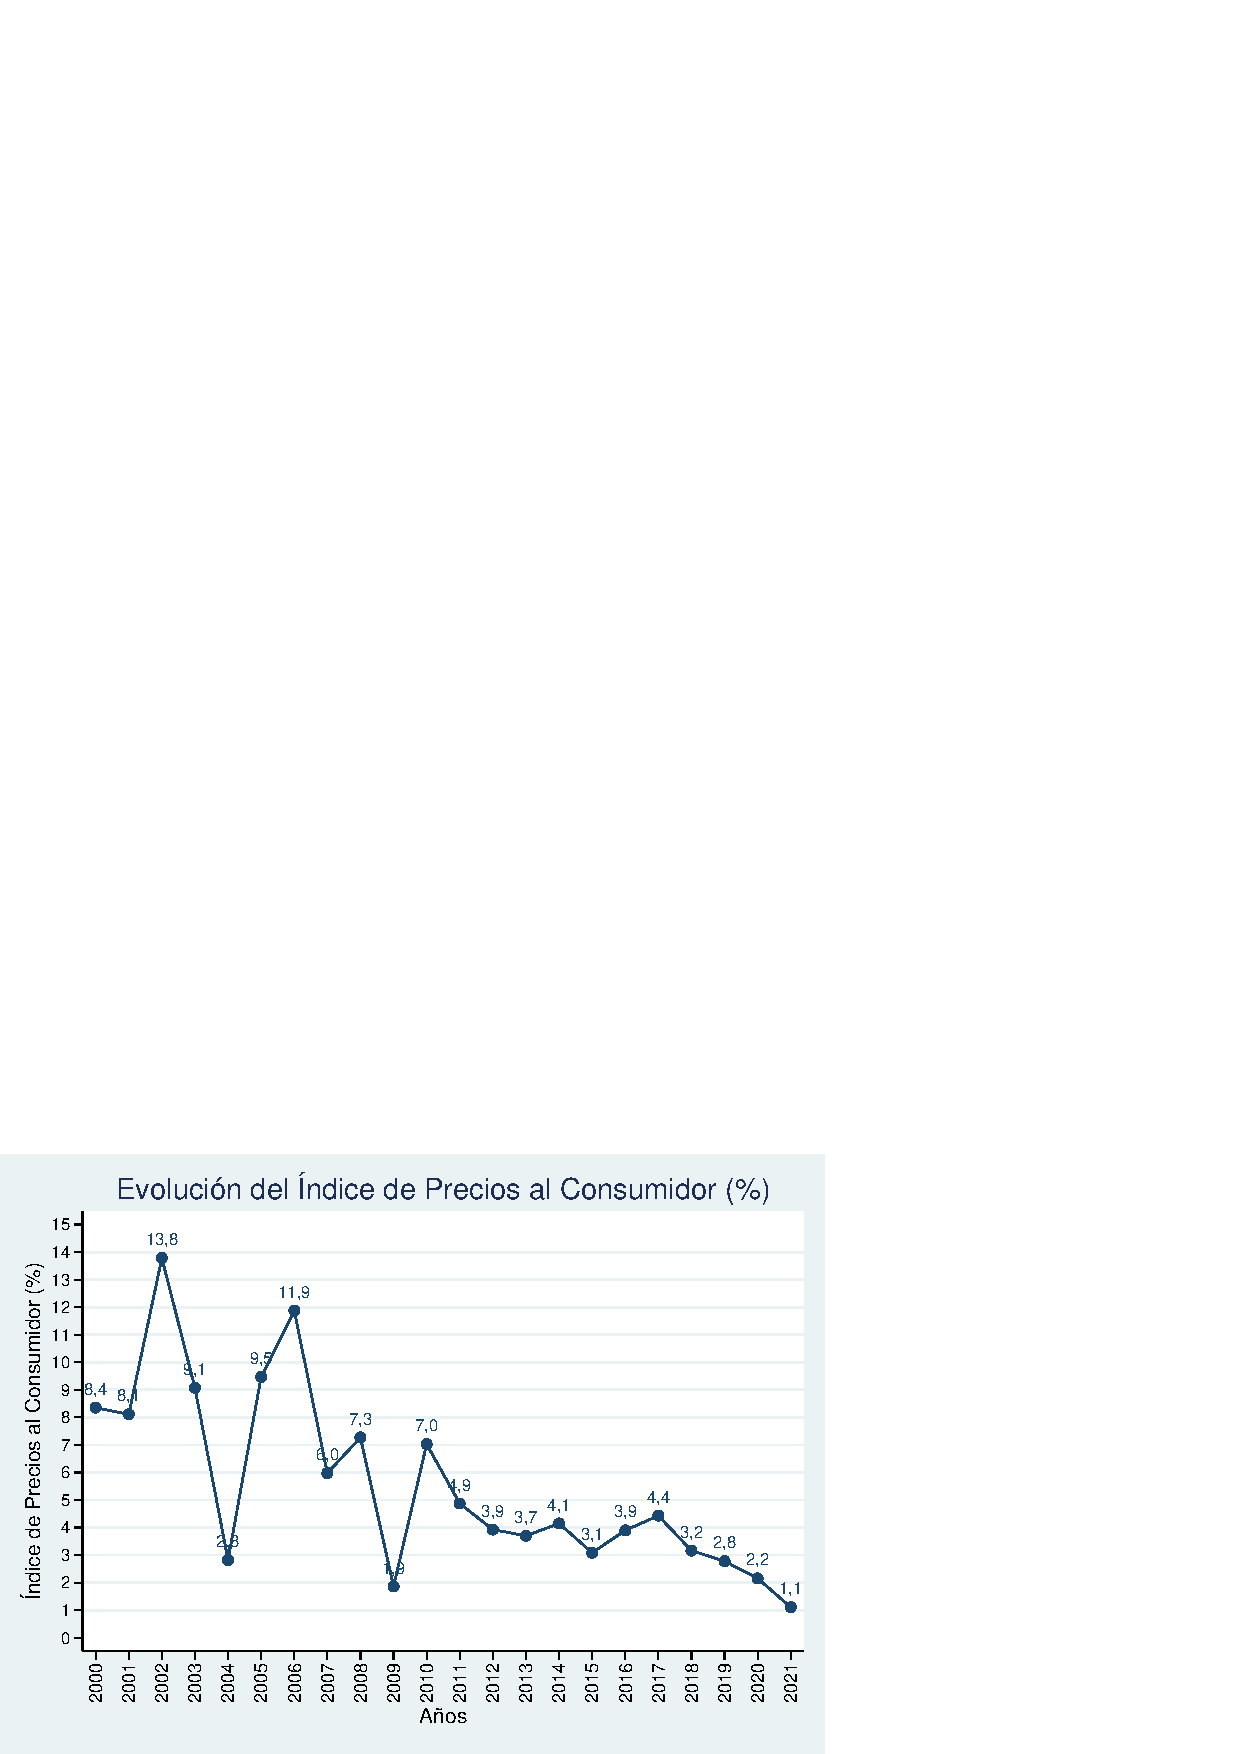
\includegraphics[scale=0.55]{BCP_ipc_year_mes.png}
                                    \item \footnotesize Fuente : Banco Central del Paraguay. 
                                    %\item \footnotesize Nota : 
                    \end{center}
\end{figure}

\subsubsection{Tasa de Interés}

Según el Informe de Estabilidad Financiera del BCP:
\textit{"Durante el año 2020, el impacto económico de la crisis sanitaria asociada a la pandemia ha debilitado a la economía mundial, regional y local".}

En este escenario, el desempeño de las variables macroeconómicas
domésticas fue afectado negativamente por la propagación del COVID-19 y
las medidas de confinamiento implementadas desde finales del primer
trimestre del año 2020 y que, posteriormente fue ron flexibilizadas a
través de una cuarentena inteligente que fue liberando y poniendo en
marcha nuevamente a los sectores económicos.

En el sector financiero, la serie de medidas adoptadas por el BCP para
asegurar la provisión de la liquidez al sistema financiero, mantener el
flujo de crédito y la continuidad de las operaciones de pagos de la
economía, han contribuido con la reactivac ión económica.

Además, en materia de política crediticia se han flexibilizado algunas
reglamentaciones a fin de proporcionar un alivio a la carga financiera
de las empresas y los hogares. Estas medidas han incluido la
reprogramación de créditos, de tal manera a evitar el deterioro de la
clasificación crediticia del cliente, de manera a que pueda seguir
siendo sujeto de crédito, y la facilidad, para las entidades
financieras, de que los cargos generados por las previsiones sean
reconocidos gradualmente en los estados de resultados.

En consecuencia, conforme se esperaba, la cartera renegociada ha
aumentado significativamente. En cuanto a la solvencia, el sistema
financiero no ha enfrentado sobresaltos, considerando que los
indicadores siguen ubicándose, con holgura, por encima de l os
requerimientos mínimos de capital.

Por su parte, la rentabilidad de las entidades ha sido adversamente
afectada, lo que se constata con la disminución del diferencial de tasas
de interés y los ratios ROA(Rentabilidad sobre activos) y ROE (
Rentabilidad sobre patrimonio neto).

La Carta Orgánica del IPS establece que la inversión de los recursos se
debe realizar en las mejores condiciones de seguridad, plazo, garantía y
rendimiento. Adicionalmente establece que los fondos destinados a
inversiones financieras deberán tener un r endimiento similar al de las
tasas pasivas de interés vigentes en el sistema bancario en el momento
de formalizarse la operación, y estarán orientados principalmente a
apoyar el sector productivo.

Al no encontrarse fácilmente tasas referenciales de mercado para un
instrumento financiero contra el cual comparar, ejemplo, un bono emitido
por una entidad financiera de segundo piso, se consideran los demás
elementos (seguridad y garantía), para llega r a conclusiones de sentido
común sobre el peso de estos elementos en cada instrumento de inversión
versus el nivel de tasa (mayor o menor) ofrecida por el mercado a una
fecha determinada y por plazos más o menos similares.

También es importante considerar que las colocaciones que realiza el IPS
en el sistema financiero son principalmente en Certificados de Depósitos
de Ahorro (CDA), lo cual es realizado mediante un sistema competitivo de
ofertas entre todas las institucio nes financieras que cumplan con
ciertos requerimientos de solvencia. Y las tasas aceptadas son por lo
menos iguales al promedio ponderado de tasas publicadas por el BCP del
sistema financiero por plazo y moneda, siendo el promedio de
rentabilidad para d icho instrumento superior a la media de mercado.

\begin{table}[H]
\begin{center}
\caption{\bf{Tasas efectivas de interés. Periodo 2011-2021}}
\begin{tabular}{l|rrrrrr}
\scriptsize
\begin{tabular}{lllllllllllll}
\cline{1-13}
\multicolumn{1}{c}{} &
  \multicolumn{12}{|c}{Mes} \\
\multicolumn{1}{c}{} &
  \multicolumn{1}{|r}{Ene} &
  \multicolumn{1}{r}{Feb} &
  \multicolumn{1}{r}{Mar} &
  \multicolumn{1}{r}{Abr} &
  \multicolumn{1}{r}{May} &
  \multicolumn{1}{r}{Jun} &
  \multicolumn{1}{r}{Jul} &
  \multicolumn{1}{r}{Ago} &
  \multicolumn{1}{r}{Sep} &
  \multicolumn{1}{r}{Oct} &
  \multicolumn{1}{r}{Nov} &
  \multicolumn{1}{r}{Dic} \\
\cline{1-13}
\multicolumn{1}{l}{Año} &
  \multicolumn{1}{|r}{} &
  \multicolumn{1}{r}{} &
  \multicolumn{1}{r}{} &
  \multicolumn{1}{r}{} &
  \multicolumn{1}{r}{} &
  \multicolumn{1}{r}{} &
  \multicolumn{1}{r}{} &
  \multicolumn{1}{r}{} &
  \multicolumn{1}{r}{} &
  \multicolumn{1}{r}{} &
  \multicolumn{1}{r}{} &
  \multicolumn{1}{r}{} \\
\multicolumn{1}{l}{\hspace{1em}2011} &
  \multicolumn{1}{|r}{10,51} &
  \multicolumn{1}{r}{11,18} &
  \multicolumn{1}{r}{11,54} &
  \multicolumn{1}{r}{12,64} &
  \multicolumn{1}{r}{13,38} &
  \multicolumn{1}{r}{13,07} &
  \multicolumn{1}{r}{12,84} &
  \multicolumn{1}{r}{12,00} &
  \multicolumn{1}{r}{12,06} &
  \multicolumn{1}{r}{12,39} &
  \multicolumn{1}{r}{12,48} &
  \multicolumn{1}{r}{12,82} \\
\multicolumn{1}{l}{\hspace{1em}2012} &
  \multicolumn{1}{|r}{12,21} &
  \multicolumn{1}{r}{11,88} &
  \multicolumn{1}{r}{11,78} &
  \multicolumn{1}{r}{12,23} &
  \multicolumn{1}{r}{12,44} &
  \multicolumn{1}{r}{12,57} &
  \multicolumn{1}{r}{12,65} &
  \multicolumn{1}{r}{13,04} &
  \multicolumn{1}{r}{12,63} &
  \multicolumn{1}{r}{12,77} &
  \multicolumn{1}{r}{12,53} &
  \multicolumn{1}{r}{12,10} \\
\multicolumn{1}{l}{\hspace{1em}2013} &
  \multicolumn{1}{|r}{12,52} &
  \multicolumn{1}{r}{12,73} &
  \multicolumn{1}{r}{12,28} &
  \multicolumn{1}{r}{11,42} &
  \multicolumn{1}{r}{11,23} &
  \multicolumn{1}{r}{11,16} &
  \multicolumn{1}{r}{11,27} &
  \multicolumn{1}{r}{11,12} &
  \multicolumn{1}{r}{10,84} &
  \multicolumn{1}{r}{10,91} &
  \multicolumn{1}{r}{11,31} &
  \multicolumn{1}{r}{11,49} \\
\multicolumn{1}{l}{\hspace{1em}2014} &
  \multicolumn{1}{|r}{10,62} &
  \multicolumn{1}{r}{10,60} &
  \multicolumn{1}{r}{11,07} &
  \multicolumn{1}{r}{10,65} &
  \multicolumn{1}{r}{10,45} &
  \multicolumn{1}{r}{10,10} &
  \multicolumn{1}{r}{9,29} &
  \multicolumn{1}{r}{9,10} &
  \multicolumn{1}{r}{8,21} &
  \multicolumn{1}{r}{8,95} &
  \multicolumn{1}{r}{8,74} &
  \multicolumn{1}{r}{8,96} \\
\multicolumn{1}{l}{\hspace{1em}2015} &
  \multicolumn{1}{|r}{8,82} &
  \multicolumn{1}{r}{9,19} &
  \multicolumn{1}{r}{9,07} &
  \multicolumn{1}{r}{8,56} &
  \multicolumn{1}{r}{8,64} &
  \multicolumn{1}{r}{8,66} &
  \multicolumn{1}{r}{8,52} &
  \multicolumn{1}{r}{8,46} &
  \multicolumn{1}{r}{8,84} &
  \multicolumn{1}{r}{8,71} &
  \multicolumn{1}{r}{9,23} &
  \multicolumn{1}{r}{9,63} \\
\multicolumn{1}{l}{\hspace{1em}2016} &
  \multicolumn{1}{|r}{10,15} &
  \multicolumn{1}{r}{10,02} &
  \multicolumn{1}{r}{10,09} &
  \multicolumn{1}{r}{10,45} &
  \multicolumn{1}{r}{10,07} &
  \multicolumn{1}{r}{9,94} &
  \multicolumn{1}{r}{9,66} &
  \multicolumn{1}{r}{9,25} &
  \multicolumn{1}{r}{9,33} &
  \multicolumn{1}{r}{9,20} &
  \multicolumn{1}{r}{9,21} &
  \multicolumn{1}{r}{8,57} \\
\multicolumn{1}{l}{\hspace{1em}2017} &
  \multicolumn{1}{|r}{9,10} &
  \multicolumn{1}{r}{8,73} &
  \multicolumn{1}{r}{8,90} &
  \multicolumn{1}{r}{8,40} &
  \multicolumn{1}{r}{8,57} &
  \multicolumn{1}{r}{8,24} &
  \multicolumn{1}{r}{8,11} &
  \multicolumn{1}{r}{7,62} &
  \multicolumn{1}{r}{7,54} &
  \multicolumn{1}{r}{7,41} &
  \multicolumn{1}{r}{7,58} &
  \multicolumn{1}{r}{7,81} \\
\multicolumn{1}{l}{\hspace{1em}2018} &
  \multicolumn{1}{|r}{7,75} &
  \multicolumn{1}{r}{7,94} &
  \multicolumn{1}{r}{7,86} &
  \multicolumn{1}{r}{7,82} &
  \multicolumn{1}{r}{7,51} &
  \multicolumn{1}{r}{7,64} &
  \multicolumn{1}{r}{7,72} &
  \multicolumn{1}{r}{7,62} &
  \multicolumn{1}{r}{7,67} &
  \multicolumn{1}{r}{8,39} &
  \multicolumn{1}{r}{8,14} &
  \multicolumn{1}{r}{8,58} \\
\multicolumn{1}{l}{\hspace{1em}2019} &
  \multicolumn{1}{|r}{8,26} &
  \multicolumn{1}{r}{8,34} &
  \multicolumn{1}{r}{9,26} &
  \multicolumn{1}{r}{8,33} &
  \multicolumn{1}{r}{8,45} &
  \multicolumn{1}{r}{8,52} &
  \multicolumn{1}{r}{8,10} &
  \multicolumn{1}{r}{8,14} &
  \multicolumn{1}{r}{7,98} &
  \multicolumn{1}{r}{8,08} &
  \multicolumn{1}{r}{7,54} &
  \multicolumn{1}{r}{7,68} \\
\multicolumn{1}{l}{\hspace{1em}2020} &
  \multicolumn{1}{|r}{7,26} &
  \multicolumn{1}{r}{7,09} &
  \multicolumn{1}{r}{7,14} &
  \multicolumn{1}{r}{7,20} &
  \multicolumn{1}{r}{7,16} &
  \multicolumn{1}{r}{7,38} &
  \multicolumn{1}{r}{6,44} &
  \multicolumn{1}{r}{6,58} &
  \multicolumn{1}{r}{6,10} &
  \multicolumn{1}{r}{5,66} &
  \multicolumn{1}{r}{5,87} &
  \multicolumn{1}{r}{5,91} \\
\multicolumn{1}{l}{\hspace{1em}2021} &
  \multicolumn{1}{|r}{6,11} &
  \multicolumn{1}{r}{5,91} &
  \multicolumn{1}{r}{5,91} &
  \multicolumn{1}{r}{6,12} &
  \multicolumn{1}{r}{} &
  \multicolumn{1}{r}{} &
  \multicolumn{1}{r}{} &
  \multicolumn{1}{r}{} &
  \multicolumn{1}{r}{} &
  \multicolumn{1}{r}{} &
  \multicolumn{1}{r}{} &
  \multicolumn{1}{r}{} \\
\cline{1-13}
\end{tabular}

\end{tabular}
                    \item \footnotesize Fuente : Banco Central del Paraguay. 
                    %\item \footnotesize Nota : 
\end{center}
\end{table}

\begin{figure}[H]
\begin{center}
                    \caption{Promedio de tasa de interés anual nominal. Periodo 2017-2020}
                    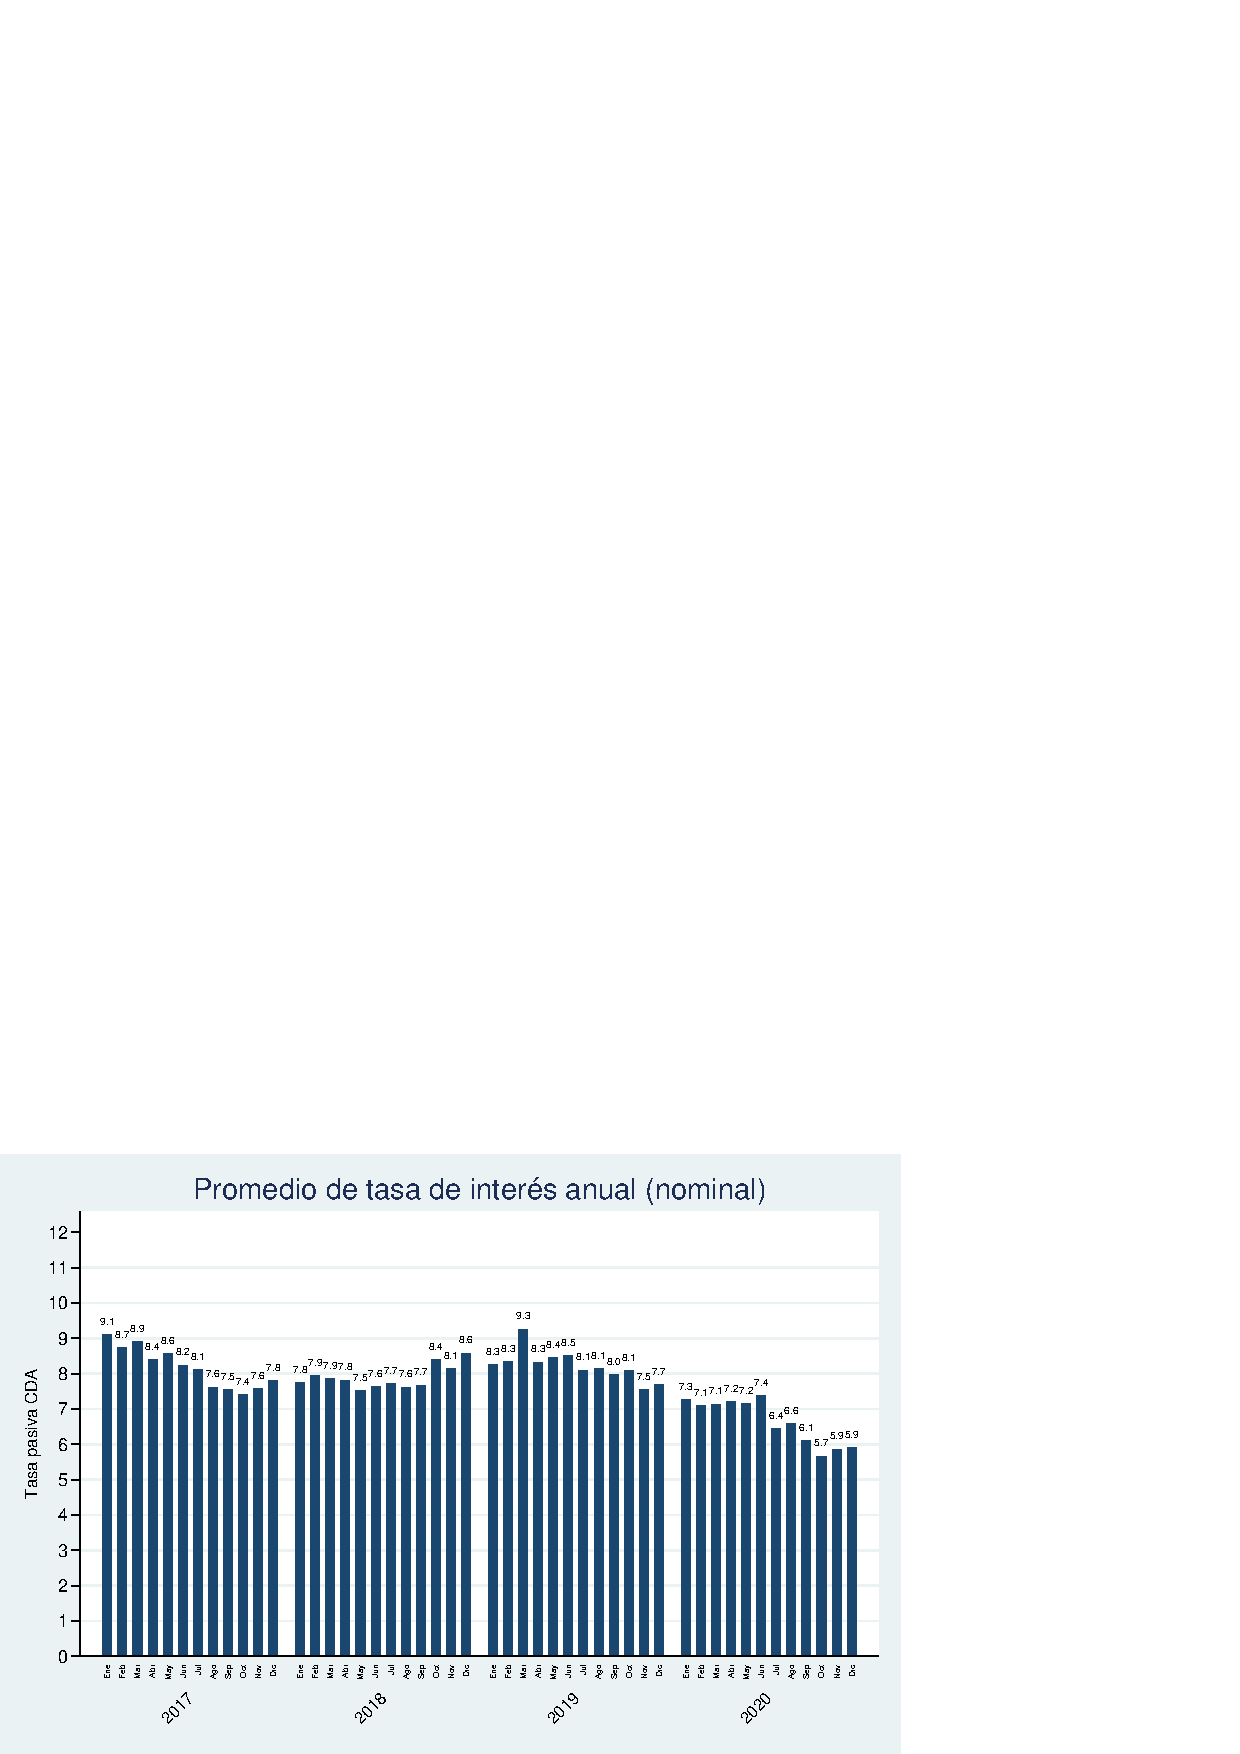
\includegraphics[scale=0.55]{BCP_tasas_pasivas.png}
                                    \item \footnotesize Fuente : Banco Central del Paraguay. 
                                    %\item \footnotesize Nota : 
                    \end{center}
\end{figure}

\subsubsection{Salario Mínimo Legal}

La remuneración mínima o el Salario Mínimo Legal (SML) es la cantidad
mínima de dinero que se le paga a un trabajador en un determinado país y
a través de una Ley establecida oficialmente, para un determinado
período laboral (hora, día o mes), que los e mpleadores deben pagar a
sus trabajadores por sus labores.

Desde el mes de julio del año 2017 se registró un cambio en la
metodología para la determinación del SML con la entrada en vigencia de
la Ley 5764/16 que modifica el Art. 255 del Código del Trabajo, la cual
establece en su artículo 1°:

\textit{"La consideración del salario mínimo será efectuada por el Poder Ejecutivo a propuesta del Consejo Nacional de Salarios Mínimos (CONASAM), sobre la base de la variación interanual del Índice de Precios al Consumidor (IPC) y su impacto en la econ
omía nacional, al mes de junio de cada año". "En los casos de profunda alteración de las condiciones macroeconómicas y financieras o de elevadas tasas de inflación, el Consejo Nacional de Salarios Mínimos podrá reunirse en un periodo distinto al indicad
o anteriormente, y considerará para la fijación del porcentaje del reajuste, los  informes sobre la inflación y la situación económica y financiera del Banco Central del Paraguay y del Ministerio de Hacienda, como así también, las perspectivas o proyecc
iones inflacionarias y económicas respectivas".}

Resulta importante destacar que, con la nueva metodología de ajuste del
Salario Mínimo Legal, lo que se pretende es compensar la pérdida del
poder adquisitivo cada año, no es una suba de salario, sino una
compensación.

Desde el 1 de julio del corriente año entró en vigencia el Decreto N°
5562/21 emitido por el Poder Ejecutivo, en el cual se oficializa el
aumento del salario mínimo en un 4,4\% ascendiendo a Gs. 2.289.324.

Al observar la evolución del SML desde abril de 2005 a junio de 2021, se
aprecia que en los últimos 5 años los niveles de variación se han
mantenido en promedio alrededor del 5\%.

\textbf{****se podría agregar la variación a la Figura 28 y el aumento del SML a Gs. 2.289.324 para el año 2021****}

\begin{figure}[H]
\begin{center}
                    \caption{Evolución del Salario Mínimo Legal. Periodo 2000-2020}
                    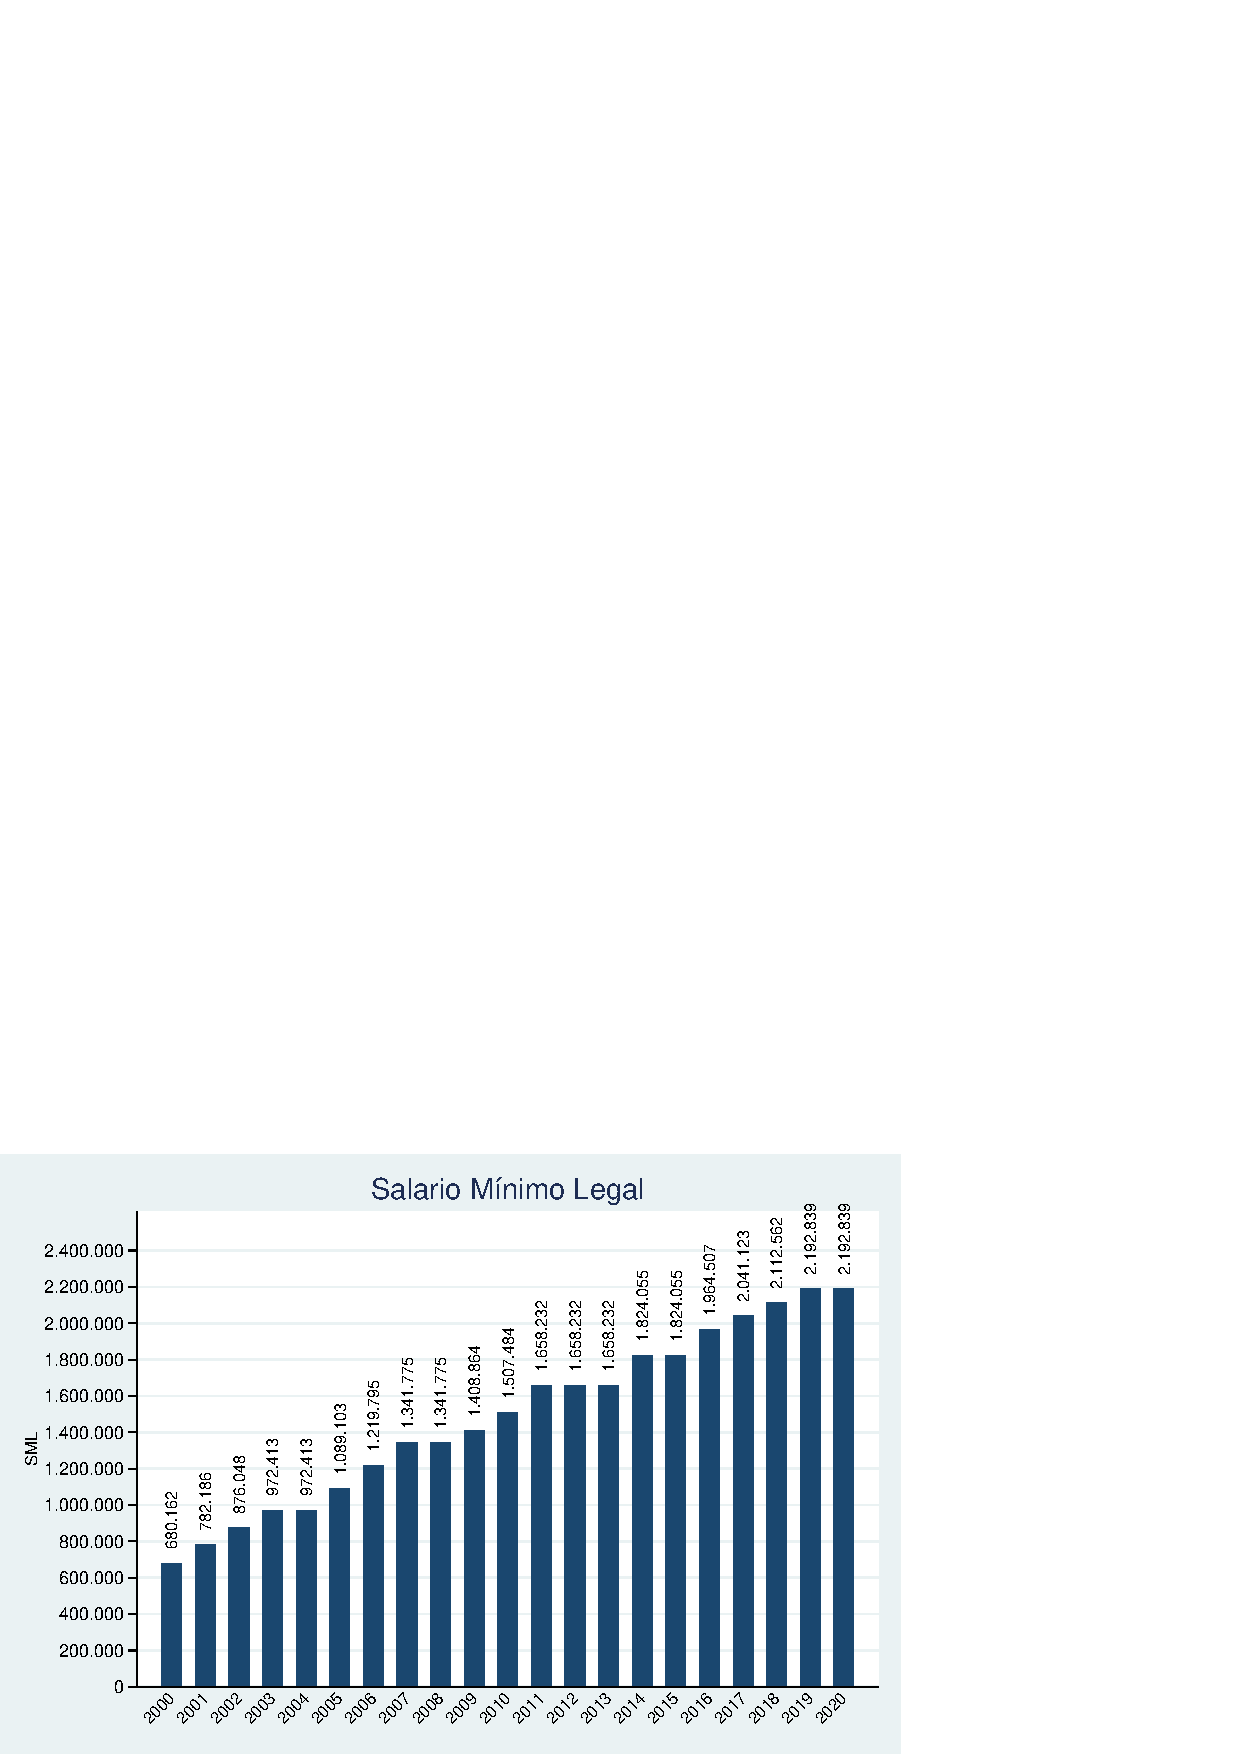
\includegraphics[scale=0.55]{BCP_sml.png}
                                    \item \footnotesize Fuente : Banco Central del Paraguay. 
                                    \item \footnotesize Nota : El SML máximo de enero a diciembre de cada año
                    \end{center}
\end{figure}

\subsubsection{Participación de las remuneraciones en el PIB}

La participación de las remuneraciones en el PIB es un indicador de la
pérdida o ganancia de las remuneraciones laborales en el reparto de la
riqueza generada.

Al observar la evolución de la tasa de participación de las
remuneraciones en el PIB desde el año 2008 al año 2019 se aprecia que si
bien hubo altibajos a lo largo del periodo considerado, la tasa se
estabilizó en torno al 32,5\%.

\begin{table}[H]
\begin{center}
\caption{\bf{Remuneración de asalariados y participación con respecto al PIB. Periodo 2008-2019}}
\begin{tabular}{l|rrrrrr}
\scriptsize
\begin{tabular}{llll}
\cline{1-4}
\multicolumn{1}{c}{} &
  \multicolumn{1}{|r}{Remuneración de asalariados} &
  \multicolumn{1}{r}{PIB (corriente)} &
  \multicolumn{1}{r}{Participación (\%)} \\
\cline{1-4}
\multicolumn{1}{l}{Año} &
  \multicolumn{1}{|r}{} &
  \multicolumn{1}{r}{} &
  \multicolumn{1}{r}{} \\
\multicolumn{1}{l}{\hspace{1em}2008} &
  \multicolumn{1}{|r}{29.448.579,54} &
  \multicolumn{1}{r}{107.403.590,63} &
  \multicolumn{1}{r}{27,42} \\
\multicolumn{1}{l}{\hspace{1em}2009} &
  \multicolumn{1}{|r}{32.625.523,04} &
  \multicolumn{1}{r}{111.030.933,59} &
  \multicolumn{1}{r}{29,38} \\
\multicolumn{1}{l}{\hspace{1em}2010} &
  \multicolumn{1}{|r}{36.976.999,49} &
  \multicolumn{1}{r}{129.092.883,48} &
  \multicolumn{1}{r}{28,64} \\
\multicolumn{1}{l}{\hspace{1em}2011} &
  \multicolumn{1}{|r}{41.443.812,37} &
  \multicolumn{1}{r}{141.486.449,39} &
  \multicolumn{1}{r}{29,29} \\
\multicolumn{1}{l}{\hspace{1em}2012} &
  \multicolumn{1}{|r}{47.214.005,92} &
  \multicolumn{1}{r}{147.225.506,09} &
  \multicolumn{1}{r}{32,07} \\
\multicolumn{1}{l}{\hspace{1em}2013} &
  \multicolumn{1}{|r}{52.209.789,29} &
  \multicolumn{1}{r}{166.350.805,11} &
  \multicolumn{1}{r}{31,39} \\
\multicolumn{1}{l}{\hspace{1em}2014} &
  \multicolumn{1}{|r}{56.662.240,64} &
  \multicolumn{1}{r}{180.174.060,97} &
  \multicolumn{1}{r}{31,45} \\
\multicolumn{1}{l}{\hspace{1em}2015} &
  \multicolumn{1}{|r}{60.164.504,04} &
  \multicolumn{1}{r}{188.477.326,98} &
  \multicolumn{1}{r}{31,92} \\
\multicolumn{1}{l}{\hspace{1em}2016} &
  \multicolumn{1}{|r}{64.338.954,09} &
  \multicolumn{1}{r}{204.647.273,08} &
  \multicolumn{1}{r}{31,44} \\
\multicolumn{1}{l}{\hspace{1em}2017} &
  \multicolumn{1}{|r}{67.329.449,45} &
  \multicolumn{1}{r}{219.122.277,20} &
  \multicolumn{1}{r}{30,73} \\
\multicolumn{1}{l}{\hspace{1em}2018} &
  \multicolumn{1}{|r}{72.961.029,38} &
  \multicolumn{1}{r}{230.576.477,47} &
  \multicolumn{1}{r}{31,64} \\
\multicolumn{1}{l}{\hspace{1em}2019} &
  \multicolumn{1}{|r}{76.770.449,53} &
  \multicolumn{1}{r}{236.566.703,63} &
  \multicolumn{1}{r}{32,45} \\
\cline{1-4}
\end{tabular}

\end{tabular}
                    \item \footnotesize Fuente : Banco Central del Paraguay. 
                    %\item \footnotesize Nota : 
\end{center}
\end{table}

\begin{figure}[H]
\begin{center}
                    \caption{Evolución de las remuneraciones en el PIB. Periodo 2008-2019}
                    \includegraphics[scale=0.55]{BCP_particRemuneraciones.png}
                                    \item \footnotesize Fuente : Banco Central del Paraguay.        %\item \footnotesize Nota : 
                    \end{center}
\end{figure}
